\begin{tikzpicture}
\definecolor{incorrect}{RGB}{255,51,76}
\definecolor{correct}{RGB}{63,188,157}

\node[inner sep=0pt] at (-7.8, 0) {A)};

\node[inner sep=0pt] at (-7.0, 0.52) {\scriptsize GT};
\node[fill=incorrect, inner sep=1.5pt] at (-7.0, 0.22) {\scriptsize NOK};

\node[inner sep=0pt] at (-7.0, -0.18) {\scriptsize Model};
\node[fill=correct, inner sep=1.5pt] at (-7.0, -0.48) {\scriptsize OK};

\node[inner sep=0pt] at (-5.2,0)
{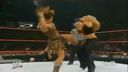
\includegraphics[width=2.4cm]{img/transnetv2/example_detections/0EXCdXUN_fk_001_07058.jpg}};
\node[inner sep=0pt] at (-2.6,0)
{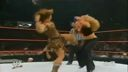
\includegraphics[width=2.4cm]{img/transnetv2/example_detections/0EXCdXUN_fk_001_07059.jpg}};
\node[inner sep=0pt] at (0,0)
{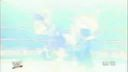
\includegraphics[width=2.4cm]{img/transnetv2/example_detections/0EXCdXUN_fk_001_07060.jpg}};
\node[inner sep=0pt] at (2.6,0)
{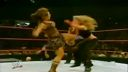
\includegraphics[width=2.4cm]{img/transnetv2/example_detections/0EXCdXUN_fk_001_07061.jpg}};
\node[inner sep=0pt] at (5.2,0)
{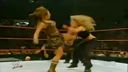
\includegraphics[width=2.4cm]{img/transnetv2/example_detections/0EXCdXUN_fk_001_07062.jpg}};

\draw[-{to reversed[scale=.4]}, thick] (-6.4, -0.85) -- (-2.6, -0.85);
\draw[{to reversed[scale=.4]}-, thick] (0, -0.85) -- (6.4, -0.85);

\draw[dotted] (-6.4, -1) -- (6.4, -1);

\node at (0, -1.1) {};
\end{tikzpicture}



\begin{tikzpicture}
\definecolor{incorrect}{RGB}{255,51,76}
\definecolor{correct}{RGB}{63,188,157}

\node[inner sep=0pt] at (-7.8, 0) {A)};

\node[inner sep=0pt] at (-7.0, 0.52) {\scriptsize GT};
\node[fill=incorrect, inner sep=1.5pt] at (-7.0, 0.22) {\scriptsize NOK};

\node[inner sep=0pt] at (-7.0, -0.18) {\scriptsize Model};
\node[fill=correct, inner sep=1.5pt] at (-7.0, -0.48) {\scriptsize OK};


\node[inner sep=0pt] at (-5.2,0)
{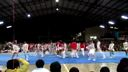
\includegraphics[width=2.4cm]{img/transnetv2/example_detections/Zoj_-rPnxGw_000_00144.jpg}};
\node[inner sep=0pt] at (-2.6,0)
{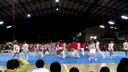
\includegraphics[width=2.4cm]{img/transnetv2/example_detections/Zoj_-rPnxGw_000_00145.jpg}};
\node[inner sep=0pt] at (0,0)
{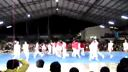
\includegraphics[width=2.4cm]{img/transnetv2/example_detections/Zoj_-rPnxGw_000_00146.jpg}};
\node[inner sep=0pt] at (2.6,0)
{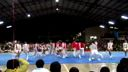
\includegraphics[width=2.4cm]{img/transnetv2/example_detections/Zoj_-rPnxGw_000_00147.jpg}};
\node[inner sep=0pt] at (5.2,0)
{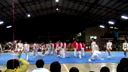
\includegraphics[width=2.4cm]{img/transnetv2/example_detections/Zoj_-rPnxGw_000_00148.jpg}};

\draw[-{to reversed[scale=.4]}, thick] (-6.4, -0.85) -- (-2.6, -0.85);
\draw[{to reversed[scale=.4]}-, thick] (0, -0.85) -- (6.4, -0.85);

\draw[dotted] (-6.4, -1) -- (6.4, -1);

\node at (0, -1.1) {};

\end{tikzpicture}

\begin{tikzpicture}
\definecolor{incorrect}{RGB}{255,51,76}
\definecolor{correct}{RGB}{63,188,157}

\node[inner sep=0pt] at (-7.8, 0) {A)};

\node[inner sep=0pt] at (-7.0, 0.52) {\scriptsize GT};
\node[fill=correct, inner sep=1.5pt] at (-7.0, 0.22) {\scriptsize OK};

\node[inner sep=0pt] at (-7.0, -0.18) {\scriptsize Model};
\node[fill=incorrect, inner sep=1.5pt] at (-7.0, -0.48) {\scriptsize NOK};



\node[inner sep=0pt] at (-5.2,0)
{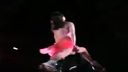
\includegraphics[width=2.4cm]{img/transnetv2/example_detections/7v_BpmoGuPI_000_02058.jpg}};
\node[inner sep=0pt] at (-2.6,0)
{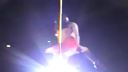
\includegraphics[width=2.4cm]{img/transnetv2/example_detections/7v_BpmoGuPI_000_02059.jpg}};
\node[inner sep=0pt] at (0,0)
{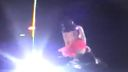
\includegraphics[width=2.4cm]{img/transnetv2/example_detections/7v_BpmoGuPI_000_02063.jpg}};
\node[inner sep=0pt] at (2.6,0)
{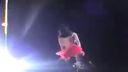
\includegraphics[width=2.4cm]{img/transnetv2/example_detections/7v_BpmoGuPI_000_02067.jpg}};
\node[inner sep=0pt] at (5.2,0)
{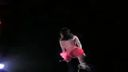
\includegraphics[width=2.4cm]{img/transnetv2/example_detections/7v_BpmoGuPI_000_02069.jpg}};

\draw[thick] (-6.4, -0.85) -- (6.4, -0.85);

\draw[dotted] (-6.4, -1) -- (6.4, -1);

\draw[line width=0.05cm] (-4.6, -1) -- (-3.2, -1);
\draw[line width=0.05cm] (4.6, -1) -- (3.2, -1);


\draw[] (-4.6, -0.92) -- (-4.6, -1.08);
\draw[] (-3.2, -0.92) -- (-3.2, -1.08);
\draw[] (4.6, -0.92) -- (4.6, -1.08);
\draw[] (3.2, -0.92) -- (3.2, -1.08);

\node at (0, -1.1) {};

\end{tikzpicture}


\begin{tikzpicture}
\definecolor{incorrect}{RGB}{255,51,76}
\definecolor{correct}{RGB}{63,188,157}

\node[inner sep=0pt] at (-7.8, 0) {B)};

\node[inner sep=0pt] at (-7.0, 0.52) {\scriptsize GT};
\node[fill=correct, inner sep=1.5pt] at (-7.0, 0.22) {\scriptsize OK};

\node[inner sep=0pt] at (-7.0, -0.18) {\scriptsize Model};
\node[fill=incorrect, inner sep=1.5pt] at (-7.0, -0.48) {\scriptsize NOK};


\node[inner sep=0pt] at (-5.2,0)
{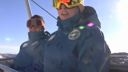
\includegraphics[width=2.4cm]{img/transnetv2/example_detections/-629gOGM1Ic_000_00286.jpg}};
\node[inner sep=0pt] at (-2.6,0)
{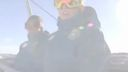
\includegraphics[width=2.4cm]{img/transnetv2/example_detections/-629gOGM1Ic_000_00289.jpg}};
\node[inner sep=0pt] at (0,0)
{
\includegraphics[width=2.4cm]{img/transnetv2/example_detections/-629gOGM1Ic_000_00291.jpg}};
\node[inner sep=0pt] at (2.6,0)
{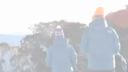
\includegraphics[width=2.4cm]{img/transnetv2/example_detections/-629gOGM1Ic_000_00294.jpg}};
\node[inner sep=0pt] at (5.2,0)
{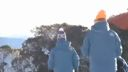
\includegraphics[width=2.4cm]{img/transnetv2/example_detections/-629gOGM1Ic_000_00296.jpg}};

\draw[-{to reversed[scale=.4]}, thick] (-6.4, -0.85) -- (-5.2, -0.85);
\draw[{to reversed[scale=.4]}-, thick] (5.2, -0.85) -- (6.4, -0.85);

\draw[dotted] (-6.4, -1) -- (6.4, -1);

\node at (0, -1.1) {};

\end{tikzpicture}


\begin{tikzpicture}
\definecolor{incorrect}{RGB}{255,51,76}
\definecolor{correct}{RGB}{63,188,157}

\node[inner sep=0pt] at (-7.8, 0) {B)};

\node[inner sep=0pt] at (-7.0, 0.52) {\scriptsize GT};
\node[fill=correct, inner sep=1.5pt] at (-7.0, 0.22) {\scriptsize OK};

\node[inner sep=0pt] at (-7.0, -0.18) {\scriptsize Model};
\node[fill=incorrect, inner sep=1.5pt] at (-7.0, -0.48) {\scriptsize NOK};



\node[inner sep=0pt] at (-5.2,0)
{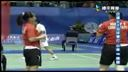
\includegraphics[width=2.4cm]{img/transnetv2/example_detections/5cUViKlaXS8_001_11719.jpg}};
\node[inner sep=0pt] at (-2.6,0)
{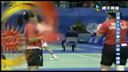
\includegraphics[width=2.4cm]{img/transnetv2/example_detections/5cUViKlaXS8_001_11723.jpg}};
\node[inner sep=0pt] at (0,0)
{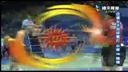
\includegraphics[width=2.4cm]{img/transnetv2/example_detections/5cUViKlaXS8_001_11730.jpg}};
\node[inner sep=0pt] at (2.6,0)
{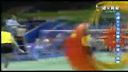
\includegraphics[width=2.4cm]{img/transnetv2/example_detections/5cUViKlaXS8_001_11740.jpg}};
\node[inner sep=0pt] at (5.2,0)
{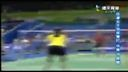
\includegraphics[width=2.4cm]{img/transnetv2/example_detections/5cUViKlaXS8_001_11745.jpg}};


\draw[-{to reversed[scale=.4]}, thick] (-6.4, -0.85) -- (-5.2, -0.85);
\draw[{to reversed[scale=.4]}-, thick] (5.2, -0.85) -- (6.4, -0.85);

\draw[dotted] (-6.4, -1) -- (6.4, -1);

\node at (0, -1.1) {};

\end{tikzpicture}

% \begin{tikzpicture}
% \definecolor{incorrect}{RGB}{255,51,76}
% \definecolor{correct}{RGB}{63,188,157}
% 
% 
% \node[inner sep=0pt] at (-7.0, 0.52) {\scriptsize GT};
% \node[fill=incorrect, inner sep=1.5pt] at (-7.0, 0.22) {\scriptsize NOK};
% 
% \node[inner sep=0pt] at (-7.0, -0.18) {\scriptsize Model};
% \node[fill=correct, inner sep=1.5pt] at (-7.0, -0.48) {\scriptsize OK};
% 
% \node[inner sep=0pt] at (-5.2,0)
% {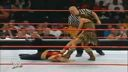
\includegraphics[width=2.4cm]{img/transnetv2/example_detections/0EXCdXUN_fk_000_06299.jpg}};
% \node[inner sep=0pt] at (-2.6,0)
% {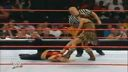
\includegraphics[width=2.4cm]{img/transnetv2/example_detections/0EXCdXUN_fk_000_06300.jpg}};
% \node[inner sep=0pt] at (0,0)
% {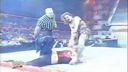
\includegraphics[width=2.4cm]{img/transnetv2/example_detections/0EXCdXUN_fk_000_06301.jpg}};
% \node[inner sep=0pt] at (2.6,0)
% {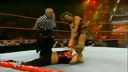
\includegraphics[width=2.4cm]{img/transnetv2/example_detections/0EXCdXUN_fk_000_06302.jpg}};
% \node[inner sep=0pt] at (5.2,0)
% {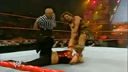
\includegraphics[width=2.4cm]{img/transnetv2/example_detections/0EXCdXUN_fk_000_06303.jpg}};
% 
% \draw[thick] (-6.4, -0.85) -- (6.4, -0.85);
% 
% \draw[dotted] (-6.4, -1) -- (6.4, -1);
% 
% \draw[line width=0.05cm] (0.6, -1) -- (2, -1);
% 
% \draw[] (0.6, -0.92) -- (0.6, -1.08);
% \draw[] (2, -0.92) -- (2, -1.08);
% 
% \node at (0, -1.1) {};
% \end{tikzpicture}

    

\begin{tikzpicture}
\definecolor{incorrect}{RGB}{255,51,76}
\definecolor{correct}{RGB}{63,188,157}

\node[inner sep=0pt] at (-7.8, 0) {C)};

\node[inner sep=0pt] at (-7.0, 0.52) {\scriptsize GT};
\node[fill=incorrect, inner sep=1.5pt] at (-7.0, 0.22) {\scriptsize NOK};

\node[inner sep=0pt] at (-7.0, -0.18) {\scriptsize Model};
\node[fill=correct, inner sep=1.5pt] at (-7.0, -0.48) {\scriptsize OK};


\node[inner sep=0pt] at (-5.2,0)
{
\includegraphics[width=2.4cm]{img/transnetv2/example_detections/1qAzo9Gdw1k_001_00965.jpg}};
\node[inner sep=0pt] at (-2.6,0)
{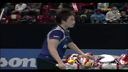
\includegraphics[width=2.4cm]{img/transnetv2/example_detections/1qAzo9Gdw1k_001_00966.jpg}};
\node[inner sep=0pt] at (0,0)
{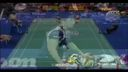
\includegraphics[width=2.4cm]{img/transnetv2/example_detections/1qAzo9Gdw1k_001_00967.jpg}};
\node[inner sep=0pt] at (2.6,0)
{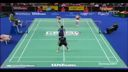
\includegraphics[width=2.4cm]{img/transnetv2/example_detections/1qAzo9Gdw1k_001_00968.jpg}};
\node[inner sep=0pt] at (5.2,0)
{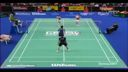
\includegraphics[width=2.4cm]{img/transnetv2/example_detections/1qAzo9Gdw1k_001_00969.jpg}};

\draw[thick] (-6.4, -0.85) -- (6.4, -0.85);

\draw[dotted] (-6.4, -1) -- (6.4, -1);

\draw[line width=0.05cm] (0.6, -1) -- (2, -1);

\draw[] (0.6, -0.92) -- (0.6, -1.08);
\draw[] (2, -0.92) -- (2, -1.08);

\node at (0, -1.1) {};

\end{tikzpicture}
    

% \begin{tikzpicture}
% \definecolor{incorrect}{RGB}{255,51,76}
% \definecolor{correct}{RGB}{63,188,157}
% 
% 
% \node[inner sep=0pt] at (-7.0, 0.52) {\scriptsize GT};
% \node[fill=incorrect, inner sep=1.5pt] at (-7.0, 0.22) {\scriptsize NOK};
% 
% \node[inner sep=0pt] at (-7.0, -0.18) {\scriptsize Model};
% \node[fill=correct, inner sep=1.5pt] at (-7.0, -0.48) {\scriptsize OK};
% 
% 
% \node[inner sep=0pt] at (-5.2,0)
% {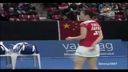
\includegraphics[width=2.4cm]{img/transnetv2/example_detections/1qAzo9Gdw1k_000_00084.jpg}};
% \node[inner sep=0pt] at (-2.6,0)
% {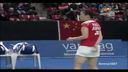
\includegraphics[width=2.4cm]{img/transnetv2/example_detections/1qAzo9Gdw1k_000_00085.jpg}};
% \node[inner sep=0pt] at (0,0)
% {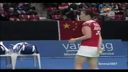
\includegraphics[width=2.4cm]{img/transnetv2/example_detections/1qAzo9Gdw1k_000_00086.jpg}};
% \node[inner sep=0pt] at (2.6,0)
% {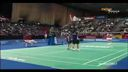
\includegraphics[width=2.4cm]{img/transnetv2/example_detections/1qAzo9Gdw1k_000_00087.jpg}};
% \node[inner sep=0pt] at (5.2,0)
% {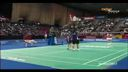
\includegraphics[width=2.4cm]{img/transnetv2/example_detections/1qAzo9Gdw1k_000_00088.jpg}};
% 
% \draw[thick] (-6.4, -0.85) -- (6.4, -0.85);
% 
% \draw[dotted] (-6.4, -1) -- (6.4, -1);
% 
% \draw[line width=0.05cm] (0.6, -1) -- (2, -1);
% 
% \draw[] (0.6, -0.92) -- (0.6, -1.08);
% \draw[] (2, -0.92) -- (2, -1.08);
% 
% \node at (0, -1.1) {};
% \end{tikzpicture}
    

    

\begin{tikzpicture}
\definecolor{incorrect}{RGB}{255,51,76}
\definecolor{correct}{RGB}{63,188,157}

\node[inner sep=0pt] at (-7.8, 0) {C)};

\node[inner sep=0pt] at (-7.0, 0.52) {\scriptsize GT};
\node[fill=correct, inner sep=1.5pt] at (-7.0, 0.22) {\scriptsize OK};

\node[inner sep=0pt] at (-7.0, -0.18) {\scriptsize Model};
\node[fill=incorrect, inner sep=1.5pt] at (-7.0, -0.48) {\scriptsize NOK};



\node[inner sep=0pt] at (-5.2,0)
{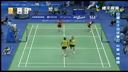
\includegraphics[width=2.4cm]{img/transnetv2/example_detections/5cUViKlaXS8_000_02242.jpg}};
\node[inner sep=0pt] at (-2.6,0)
{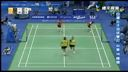
\includegraphics[width=2.4cm]{img/transnetv2/example_detections/5cUViKlaXS8_000_02244.jpg}};
\node[inner sep=0pt] at (0,0)
{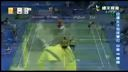
\includegraphics[width=2.4cm]{img/transnetv2/example_detections/5cUViKlaXS8_000_02245.jpg}};
\node[inner sep=0pt] at (2.6,0)
{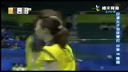
\includegraphics[width=2.4cm]{img/transnetv2/example_detections/5cUViKlaXS8_000_02246.jpg}};
\node[inner sep=0pt] at (5.2,0)
{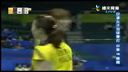
\includegraphics[width=2.4cm]{img/transnetv2/example_detections/5cUViKlaXS8_000_02248.jpg}};

\draw[-{to reversed[scale=.4]}, thick] (-6.4, -0.85) -- (-2.6, -0.85);
\draw[{to reversed[scale=.4]}-, thick] (2.6, -0.85) -- (6.4, -0.85);

\draw[dotted] (-6.4, -1) -- (6.4, -1);

\node at (0, -1.1) {};

\end{tikzpicture}

% \begin{tikzpicture}
% \definecolor{incorrect}{RGB}{255,51,76}
% \definecolor{correct}{RGB}{63,188,157}
% 
% 
% \node[inner sep=0pt] at (-7.0, 0.52) {\scriptsize GT};
% \node[fill=incorrect, inner sep=1.5pt] at (-7.0, 0.22) {\scriptsize NOK};
% 
% \node[inner sep=0pt] at (-7.0, -0.18) {\scriptsize Model};
% \node[fill=correct, inner sep=1.5pt] at (-7.0, -0.48) {\scriptsize OK};
% 
% \node[inner sep=0pt] at (-5.2,0)
% {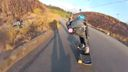
\includegraphics[width=2.4cm]{img/transnetv2/example_detections/0nZQWIxsLB8_000_01417.jpg}};
% \node[inner sep=0pt] at (-2.6,0)
% {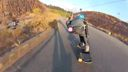
\includegraphics[width=2.4cm]{img/transnetv2/example_detections/0nZQWIxsLB8_000_01418.jpg}};
% \node[inner sep=0pt] at (0,0)
% {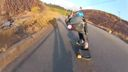
\includegraphics[width=2.4cm]{img/transnetv2/example_detections/0nZQWIxsLB8_000_01419.jpg}};
% \node[inner sep=0pt] at (2.6,0)
% {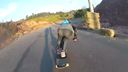
\includegraphics[width=2.4cm]{img/transnetv2/example_detections/0nZQWIxsLB8_000_01420.jpg}};
% \node[inner sep=0pt] at (5.2,0)
% {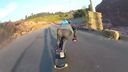
\includegraphics[width=2.4cm]{img/transnetv2/example_detections/0nZQWIxsLB8_000_01421.jpg}};
% 
% \draw[thick] (-6.4, -0.85) -- (6.4, -0.85);
% 
% \draw[dotted] (-6.4, -1) -- (6.4, -1);
% 
% \draw[line width=0.05cm] (0.6, -1) -- (2, -1);
% 
% \draw[] (0.6, -0.92) -- (0.6, -1.08);
% \draw[] (2, -0.92) -- (2, -1.08);
% 
% \node at (0, -1.1) {};
% 
% \end{tikzpicture}

\begin{tikzpicture}
\definecolor{incorrect}{RGB}{255,51,76}
\definecolor{correct}{RGB}{63,188,157}

\node[inner sep=0pt] at (-7.8, 0) {D)};

\node[inner sep=0pt] at (-7.0, 0.52) {\scriptsize GT};
\node[fill=correct, inner sep=1.5pt] at (-7.0, 0.22) {\scriptsize OK};

\node[inner sep=0pt] at (-7.0, -0.18) {\scriptsize Model};
\node[fill=incorrect, inner sep=1.5pt] at (-7.0, -0.48) {\scriptsize NOK};


\node[inner sep=0pt] at (-5.2,0)
{\includegraphics[width=2.4cm]{img/transnetv2/example_detections/0kzuXD0PmNg_000_06005.jpg}};
\node[inner sep=0pt] at (-2.6,0)
{\includegraphics[width=2.4cm]{img/transnetv2/example_detections/0kzuXD0PmNg_000_06006.jpg}};
\node[inner sep=0pt] at (0,0)
{\includegraphics[width=2.4cm]{img/transnetv2/example_detections/0kzuXD0PmNg_000_06007.jpg}};
\node[inner sep=0pt] at (2.6,0)
{\includegraphics[width=2.4cm]{img/transnetv2/example_detections/0kzuXD0PmNg_000_06008.jpg}};
\node[inner sep=0pt] at (5.2,0)
{\includegraphics[width=2.4cm]{img/transnetv2/example_detections/0kzuXD0PmNg_000_06009.jpg}};

\draw[thick] (-6.4, -0.85) -- (6.4, -0.85);

\draw[dotted] (-6.4, -1) -- (6.4, -1);

\draw[line width=0.05cm] (-0.6, -1) -- (-2, -1);

\draw[] (-0.6, -0.92) -- (-0.6, -1.08);
\draw[] (-2, -0.92) -- (-2, -1.08);

\node at (0, -1.1) {};

\end{tikzpicture}

    

\begin{tikzpicture}
\definecolor{incorrect}{RGB}{255,51,76}
\definecolor{correct}{RGB}{63,188,157}

\node[inner sep=0pt] at (-7.8, 0) {D)};

\node[inner sep=0pt] at (-7.0, 0.52) {\scriptsize GT};
\node[fill=correct, inner sep=1.5pt] at (-7.0, 0.22) {\scriptsize OK};

\node[inner sep=0pt] at (-7.0, -0.18) {\scriptsize Model};
\node[fill=incorrect, inner sep=1.5pt] at (-7.0, -0.48) {\scriptsize NOK};



\node[inner sep=0pt] at (-5.2,0)
{\includegraphics[width=2.4cm]{img/transnetv2/example_detections/-17hVQk3wXI_000_03859.jpg}};
\node[inner sep=0pt] at (-2.6,0)
{\includegraphics[width=2.4cm]{img/transnetv2/example_detections/-17hVQk3wXI_000_03861.jpg}};
\node[inner sep=0pt] at (0,0)
{\includegraphics[width=2.4cm]{img/transnetv2/example_detections/-17hVQk3wXI_000_03862.jpg}};
\node[inner sep=0pt] at (2.6,0)
{\includegraphics[width=2.4cm]{img/transnetv2/example_detections/-17hVQk3wXI_000_03863.jpg}};
\node[inner sep=0pt] at (5.2,0)
{\includegraphics[width=2.4cm]{img/transnetv2/example_detections/-17hVQk3wXI_000_03864.jpg}};

\draw[thick] (-6.4, -0.85) -- (6.4, -0.85);

\draw[dotted] (-6.4, -1) -- (6.4, -1);

\draw[line width=0.05cm] (0.6, -1) -- (2, -1);

\draw[] (0.6, -0.92) -- (0.6, -1.08);
\draw[] (2, -0.92) -- (2, -1.08);

\node at (0, -1.1) {};

\end{tikzpicture}
    
    

\begin{tikzpicture}
\definecolor{incorrect}{RGB}{255,51,76}
\definecolor{correct}{RGB}{63,188,157}
\definecolor{unknown}{RGB}{180,180,180}

\node[inner sep=0pt] at (-7.8, 0) {E)};

\node[inner sep=0pt] at (-7.0, 0.52) {\scriptsize GT};
\node[fill=unknown, inner sep=1.5pt] at (-7.0, 0.22) {\scriptsize ??};

\node[inner sep=0pt] at (-7.0, -0.18) {\scriptsize Model};
\node[fill=unknown, inner sep=1.5pt] at (-7.0, -0.48) {\scriptsize ??};


\node[inner sep=0pt] at (-5.2,0)
{\includegraphics[width=2.4cm]{img/transnetv2/example_detections/6e2-G6CXeT0_000_01253.jpg}};
\node[inner sep=0pt] at (-2.6,0)
{\includegraphics[width=2.4cm]{img/transnetv2/example_detections/6e2-G6CXeT0_000_01254.jpg}};
\node[inner sep=0pt] at (0,0)
{\includegraphics[width=2.4cm]{img/transnetv2/example_detections/6e2-G6CXeT0_000_01255.jpg}};
\node[inner sep=0pt] at (2.6,0)
{\includegraphics[width=2.4cm]{img/transnetv2/example_detections/6e2-G6CXeT0_000_01256.jpg}};
\node[inner sep=0pt] at (5.2,0)
{\includegraphics[width=2.4cm]{img/transnetv2/example_detections/6e2-G6CXeT0_000_01257.jpg}};

\draw[thick] (-6.4, -0.85) -- (6.4, -0.85);

\draw[dotted] (-6.4, -1) -- (6.4, -1);

\draw[line width=0.05cm] (0.6, -1) -- (2, -1);

\draw[] (0.6, -0.92) -- (0.6, -1.08);
\draw[] (2, -0.92) -- (2, -1.08);

\node at (0, -1.1) {};

\end{tikzpicture}

    

\begin{tikzpicture}
\definecolor{incorrect}{RGB}{255,51,76}
\definecolor{correct}{RGB}{63,188,157}
\definecolor{unknown}{RGB}{180,180,180}

\node[inner sep=0pt] at (-7.8, 0) {E)};

\node[inner sep=0pt] at (-7.0, 0.52) {\scriptsize GT};
\node[fill=unknown, inner sep=1.5pt] at (-7.0, 0.22) {\scriptsize ??};

\node[inner sep=0pt] at (-7.0, -0.18) {\scriptsize Model};
\node[fill=unknown, inner sep=1.5pt] at (-7.0, -0.48) {\scriptsize ??};

\node[inner sep=0pt] at (-5.2,0)
{\includegraphics[width=2.4cm]{img/transnetv2/example_detections/-629gOGM1Ic_001_02421.jpg}};
\node[inner sep=0pt] at (-2.6,0)
{\includegraphics[width=2.4cm]{img/transnetv2/example_detections/-629gOGM1Ic_001_02422.jpg}};
\node[inner sep=0pt] at (0,0)
{\includegraphics[width=2.4cm]{img/transnetv2/example_detections/-629gOGM1Ic_001_02423.jpg}};
\node[inner sep=0pt] at (2.6,0)
{\includegraphics[width=2.4cm]{img/transnetv2/example_detections/-629gOGM1Ic_001_02424.jpg}};
\node[inner sep=0pt] at (5.2,0)
{\includegraphics[width=2.4cm]{img/transnetv2/example_detections/-629gOGM1Ic_001_02425.jpg}};

\draw[-{to reversed[scale=.4]}, thick] (-6.4, -0.85) -- (0, -0.85);
\draw[{to reversed[scale=.4]}-, thick] (2.6, -0.85) -- (6.4, -0.85);

\draw[dotted] (-6.4, -1) -- (6.4, -1);

\node at (0, -1.1) {};

\end{tikzpicture}
